\documentclass[12pt,a4paper]{report}
\usepackage[utf8]{inputenc}
\usepackage[french]{babel}
\usepackage[T1]{fontenc}
\usepackage{graphicx}
\usepackage[left=2cm,right=2cm,top=2cm,bottom=2cm]{geometry}
\usepackage{float}


\author{Louis Lainé}
\title{SGBD}
\begin{document}

% Différentes Phases projet : 
% 1. Définition du projet
% 2. Identification des paramètres
% 3. Identification des ressources
% 4. Gestion du temps (par quoi on a commencé)
% 5. Test de l'application 


\section{Cahier des charges}
A la lecture du cahier des charges, nous avons déterminés quelles étaient les spécifications et les attentes. 

L'application devra couvrir la gestion d'une base de données minimaliste de médicaments et effets correspondants.

Elle devra répondre aux spécifications suivantes : 

\subsection*{Chargement des données}
\begin{description}
	\item La persistance des données sera assuré par un fichier \textbf{texte}. 
	\item Les données devront être chargés, une fois parsées dans l'application durant toute la durée de vie de l'application. 
\end{description}
\subsection*{Création d'une fonction d'usage}
Une fonction d'usage devra être implémenté au cas ou l'utilisateur, n'a pas appelé le programme avec les bons paramètres. 

Une fonctionnalité d'aide, accessible via un \textbf{-h} ou \textbf{-help}. 

\subsection*{Validité de la base de données}
Une exception devra être lancé, au cas ou la base de données n'est plus accessible. 

\subsection*{Histogramme}
Nécessité de créer, un histogramme des effets secondaires existant correspondant à un médicament et de pouvoir visualiser cet histogramme. 

\subsection*{Recherche d'informations}
L'application devra être en mesure, de faire plusieurs recherches sur la base de données. 
\begin{enumerate}
	\item La liste des médicaments ayant un effet secondaire, en commun. L'utilisateur saisira un effet secondaire, l'application lui renverra l'ensemble des médicaments contenant cet effet. 
	\item La liste des médicaments partageant le plus d'effet secondaires possibles avec un médicament saisi par l'utilisateur. 
	\item L'utilisateur aura accès à tous les médicaments partageant un ou plusieurs effets secondaires. Pour ce faire l'utilisation de deux algorithme, qui devront être développé : 
	\begin{itemize}
		\item Parcoure tous les médicaments et sélectionne ceux qui ont le plus d'effet. 
		\item Renvoie les deux premiers résultats trouvés avec au moins un effet secondaire identique.
	\end{itemize}
\end{enumerate}

\subsection*{Bruit et précision}
Calculer l'efficacité de l'algorithme de recherche par le biais de : 
\begin{equation}
	\frac{nbMedicamentsTrouves}{nbMedicamentsNormalementAtribues}
\end{equation}

\subsection*{Ajout de nouveau médicament}
L'utilisateur doit pouvoir ajouter un nouveau médicament
\subsection*{Interface graphique}
L'application sera livrée avec une interface graphique en plus de l'interface classique. 

\section{Identification des ressources}
Une fois le cahier des charges bien déchiffré, nous avons du déterminer le moyen par lequel les contraintes allaient être mise en oeuvre. 
Pour des raisons de flexibilité et d'évolution, nous avons décidés de développer en suivant une architecture assez spécifique. 
Cette architecture va permettre entre autres, de pouvoir changer aisement de source de fichier. 

Actuellement il est nécessaire d'utiliser un fichier texte, mais si par exemple, on change pour du XML ou du JSON il suffira uniquement de recoder la classe Parser en suivant l'interface \textbf{IParser}.
Ainsi la source de donnera changera, sans affecter le reste de l'application et restera totalement invisible pour l'utilisateur. 




L'utilisation des containers classique C++ a été utilisé pour développer cette application. 

\section{Fonctionnement}
\subsection*{Conception}
Lors de la phase de conception nous avons décidés de mettre en place une architecture trois-tiers. 
\begin{figure}[h]
	\centering
	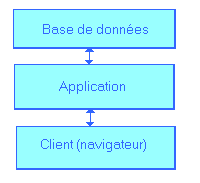
\includegraphics[width=6cm]{3tier-fr.png}
	\caption{Schema de l'architecture trois-tiers}
\end{figure}

\begin{description}
	\item[Présentation] correspondant à l'affichage, le dialogue avec l'utilisateur. 
	\item[Traitement] correspondant à la couche métier, la mise en œuvre de l'ensemble des règles de gestion et de la logique applicative
	\item[Accès aux données] correspondant aux données qui sont destinées à être conservées sur la durée, voire de manière définitive.
\end{description}

En suivant cette logique, nous avons donc conçu l'architecture suivante concernant l'application. 

Le diagramme suit la notation UML. 
\begin{figure}[H]
	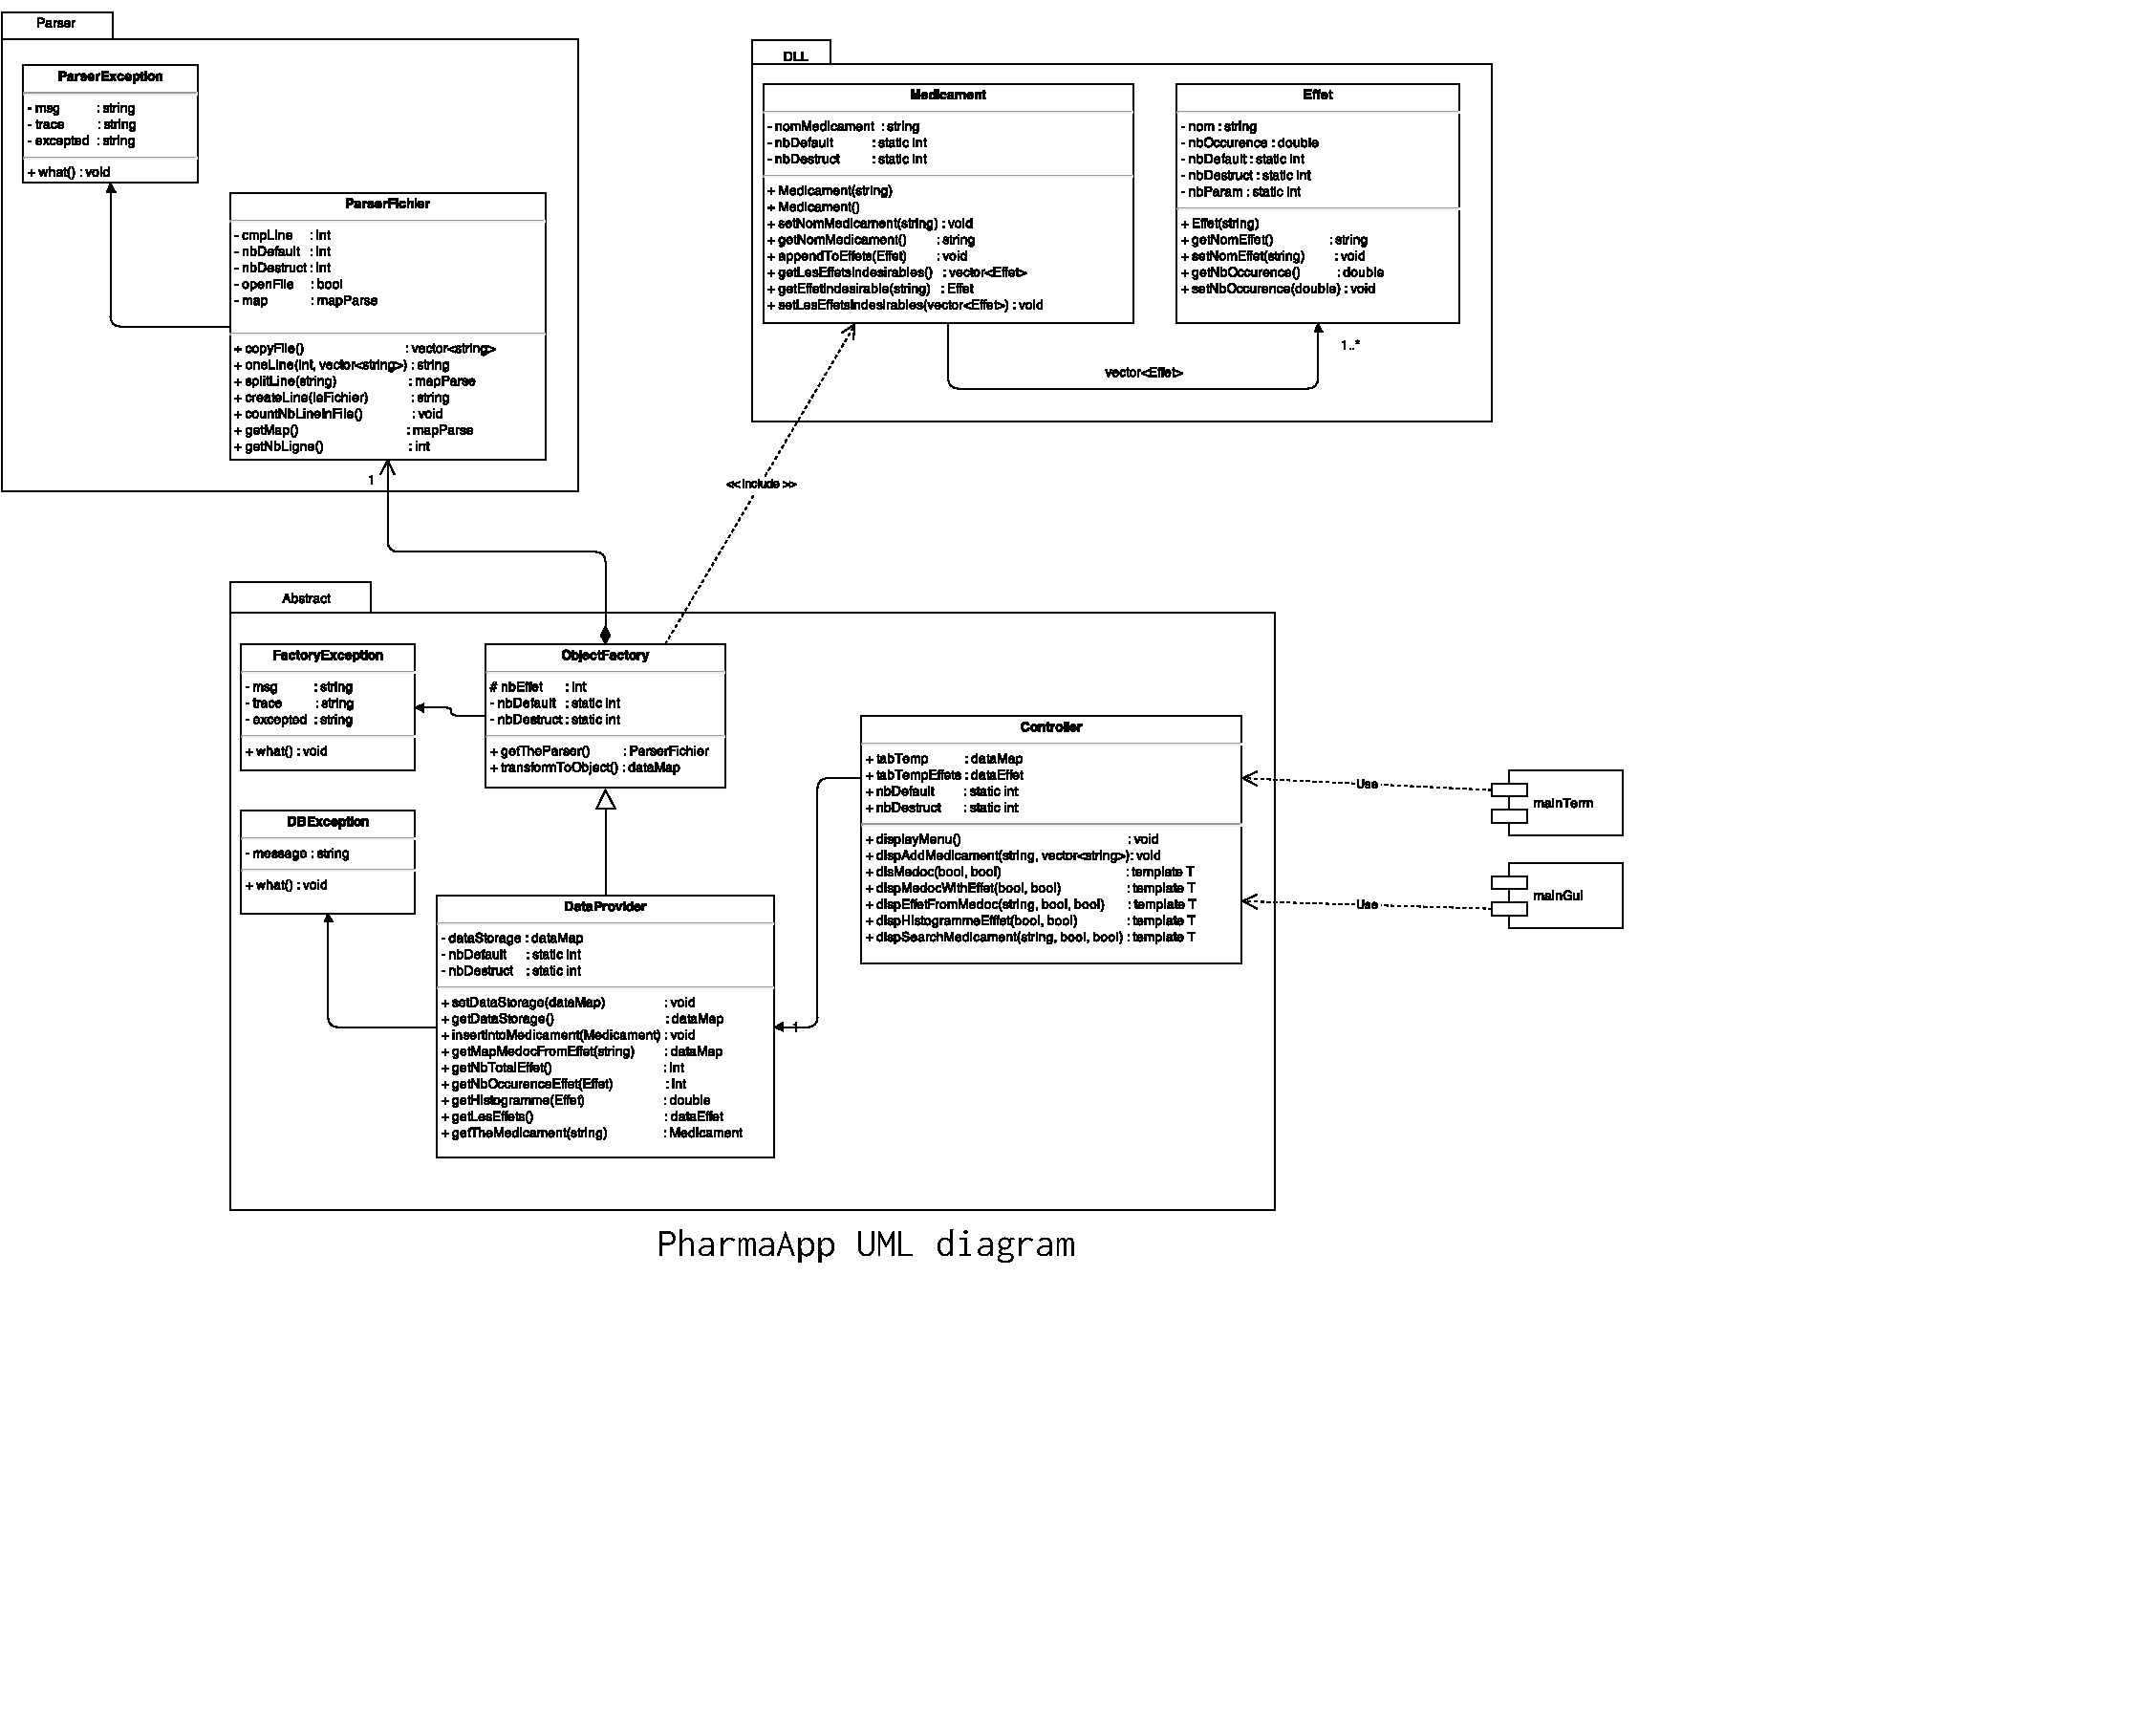
\includegraphics[scale=0.8, angle=90]{classes.pdf}
\end{figure}
\newpage
\begin{description}
	\item La couche de présentation est représenté par les modules \textbf{mainTerm} et \textbf{mainGui}
	\item La couche de traitement est représenté par les packages \textbf{Abstract} \textbf{Parser} et \textbf{Dll}, représentant la logique applicative, ainsi que l'accès à la base de données. 
	\item Les données, correspondent au fichier \textbf{liste.txt}\footnote{Non représenté sur le schéma}.
\end{description}



\subsection*{Logique métier}
\subsubsection*{ParserFichier}
\begin{verbatim}
34.	typedef std::map<string, std::vector<string> > mapParse;
35.	typedef std::map<string, std::vector<string> >::iterator mapParseIterator;
36. typedef std::vector<string> leFichier;
\end{verbatim}

C'est la classe qui va permettre la dialogue entre le fichier texte et les objets. 

Cette classe va charger les données issue du fichier texte, dans une \textit{mapParse}.

Cette map sera constitué en clé, d'un \textit{string} associé avec un \textit{vector<string>}. 
Cette conception rappelle la base de données qui à la forme suivante : 
\begin{verbatim}
nom du médicament : effet1, effet2 et effet3.
\end{verbatim}

\subsubsection*{ObjectFactory}
\begin{verbatim}
34. typedef std::map<int, Medicament> dataMap;
35. typedef std::map<string, std::vector<string> > parserMap;
\end{verbatim}

ObjectFactory, est la classe permettant la transition des données en objet. 
Cette couche, abstraite permettre de remonter les données en objet vers la couche supérieure.  

La fonction \textit{transformToObject()}, qui se base sur l'utilisation du \textit{ParserFichier}, va parcourir chaque ligne du fichier et créer les objets correspondant, à l'aide des fonctions de \textit{ParserFichier} et de la Dll pour créer les objets \textit{Médicament} et \textit{Effet}

\subsubsection*{DataProvider}
\begin{verbatim}

20. typedef std::map<int, Medicament> dataMap;
...
24. typedef std::map<string, std::vector<string> > parserMap;
...
28. typedef std::map<string, double> dataEffet;
\end{verbatim}
La couche DataProvider, héritant directement de la couche inférieure \textit{ObjectFactory}, sera considéré comme l'objet \textbf{base de données} de l'appliaction. 

Les données sont durant toute la durée de vie de l'appliaction chargé dans cet objet via un attribut privée \textit{DataProvider::dataStorage}.

Ainsi toutes les fonctions de traitements concernant les données utiliseront le \textit{DataProvider} comme source de données.

\paragraph*{Utilisation}

Lors de l'instanciation de l'objet \footnote{équivalent à la création de la base de données} la méthode mère \textit{TransformToObject()} sera appelé pour pour récupérer dans le scope les données et hydrater l'attribut \textit{DataProvider::dataStorage}. \\

\begin{verbatim}
	try{
		this->dataStorage = this->transformToObjet();
	}catch(ObjectFactory::FactoryException e){
		e.what();
	}
\end{verbatim}
Toutes les "requêtes", utiliseront cet attribut comme source de données. 

\subsubsection*{Controller}
C'est la couche d'abstraction pour la gestion des évenements. \\
Pour éviter de créer une fonction \textit{main()} à ralonge et illisible, cette classe se chargera de renvoyer en fonction d'un potentiel choix utilisateur, les données mise en forme qui pourront être affichés dans la fonction \textit{main()}, par la suite. 


Cette classe se voulant polyvalente pour une utilisation graphique ou cli, renverra en fonction d'attribut passé en paramètre dans les méthodes de, renvoyer un affichage de données ou de renvoyer les données via un \textbf{dataMap}. 

\begin{verbatim}
//Exemple d'une fonction
template <typename T>
T Controller::dispEffetFromMedoc(...) {
	//Fonction d'usage de la base de données
	try{
		this->tabTemp = this->database.getMapMedocFromEffet(theNomEffet);
	}catch(DataProvider::DBException e){
		e.getMessage();
	}
	...
	//Le renvoie utile pour l'utilisation dans un main graphique par exemple.
	if (asReturn){
		return this->tabTemp;
	}
	...
	return T();
}
\end{verbatim}

Ainsi, qu'on développe un main graphique ou cli, la classe controller sera toujours celle qui sera utilisé pour la gestion des évenements, grâce à l'utilisation de \textit{template}\footnote{concept C++}. 

\subsection{Interface Graphique}
Le cahier des charges préconisait une utilisation de QtCreator. 

Par manque de souplesse et les trop fortes contraintes imposés par Qt, nous avons décidé de ne pas utiliser cette libraire et d'utiliser une beaucoup plus puissante, \textbf{GTK} à l'aide de \textbf{GTKmm}. 


L'application n'a malheureusement pas été développé jusqu'à terme (à retrouver sur la \textbf{branch UI} du repo). 

Cependant, elle prend en compte la fonctionnalité de visualisation des médicaments avec les effets, ainsi que la recherche de médicaments ayant un effet en commun. 



\end{document}